\eat{
\begin{figure*}
    \centering
    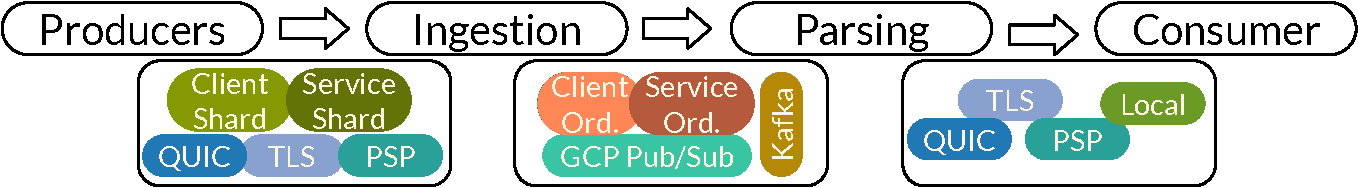
\includegraphics[width=\textwidth]{img/elk-app}
    \vspace{10pt}
    \caption{This ETL application uses three forms of communication, all supported by \name: load balancing and encryption to ingest the data and extract relevant fields, ordering primitives and different services to then transform the data into summary statistics, and finally potential fast-path optimizations to load the data for user use.}
    \label{f:elk-app}
\end{figure*}
}
\newcommand{\etlapp}{ETLApp\xspace}
\section{Application Benefits Evaluation}\label{s:applications}
In this section, we discuss implementing an ETL (extract, transform, and load) application in \name, and use it to demonstrate how \name can lower the operating cost of applications deployed in the cloud and improve their throughput and latency. We delay an evaluation of \name's abstractions to \S\ref{s:eval}. 
Our implementation of \name, as well as everything required to reproduce our results, is publicly available as we describe in Appendix~\ref{app:artifact}.

\etlapp, is a \name based application that processes streaming logs in near-realtime to produce summary statistics and metrics that can be used by users or displayed on a dashboard. \etlapp consists of four microservices:
(1) \emph{producers}, which run at the data source (\ie where logs are generated) and send logs and other telemetry information to (2) \emph{ingesters}, which perform light-weight analysis on these logs to determine how they should be ordered and then publish them to an appropriate topic in a publish-subscribe service. (3) \emph{Parsers} subscribe to these topics, parse log entries published by the ingesters, compute summary statistics and forward them to (4) \emph{consumers}, which store them and allow users or applications to query and retrieve computed statistics.

\etlapp uses a variety of communication functions and \tunnels: the producers use QUIC or TLS (and PSP~\cite{psp}, where available) to protect their communication with the ingester (\S\ref{s:app:quic}) and a load balancer \tunnel to decide what ingester the producer should send data to (\S\ref{s:app:lb}; ingesters and parsers use a Kafka~\cite{kafka} or cloud provider publish-subscribe \tunnel (\S\ref{s:app:pubsub}; and the parser uses a local communication \tunnel that minimizes encryption and transport costs (using techniques inspired by Slim~\cite{slim}) when the parser and consumer microservices are colocated on the same server.


\etlapp consists of \textasciitilde 2,300 lines of Rust code.
The \tunnels we used, which include ones implementing QUIC, TCP, UDP (via the kernel, Shenango~\cite{shenango}, and a custom DPDK datapath), TLS, ordering, four publish-subscribe services, reliability, routing, serialization, and sharding, consist of  \textasciitilde 15,000 lines of Rust code. Individual \tunnels range from \textasciitilde 400 lines for TLS and QUIC \tunnels to \textasciitilde 5,000 lines for a DPDK \tunnel.
\input{elk-kafka-gcp}

In the remainder of this section, we first evaluate \etlapp's end-to-end performance and demonstrate reconfiguration's performance benefits. After that, we describe reconfiguration in more detail for three cases: QUIC and TLS (\S\ref{s:app:quic}), publish-subscribe message queues (\S\ref{s:app:pubsub} and load balancing (\S\ref{s:app:lb}). 

\paragrapha{End-to-End Performance} We use processing latency as the main metric for evaluating \etlapp's performance. We define processing latency as the time taken between when log messages are available to the producer and when the messages are incorporated in the consumer's summary statistics. Our performance evaluation uses a fixed offered load, so processing latency accounts for both computation time and queueing.
Figure~\ref{f:elk-kafka-gcp} shows \etlapp's processing latency in two configurations: one with a Kafka~\cite{kafka} instance available in the local cluster and one without. 
Deciding whether to run a local Kafka instance or use a managed publish-subscribe service is a common choice application operators must make: running a self-hosted Kafka instance requires constant hardware resources but can be closer to other application components and tuned for the application's workload, offering better performance. Meanwhile, managed services such as GCP Pub/Sub offer a per-message cost model (see \S\ref{s:app:pubsub}) but can have lower performance. \name allows a single \etlapp implementation to work in both cases, since programmers \texttt{Select} between these two alternatives when establishing connections at the ingester and parser. We ran this evaluation on Cloudlab \texttt{m510}
machines using Linux kernel 5.15 with Microk8s version 1.27.5 as a container runtime and Kafka version 3.1.0, and used 8 ingesters and 4 parsers. For every interarrival duration, our workload adds a batch of 16 150-byte records to the producer's log for processing. Our results (Figure~\ref{f:elk-kafka-gcp}) show that using a Kafka \tunnel enables lower processing latency for \etlapp at higher offered loads (or lower interarrival times). 
However, at lower offered loads using the GCP Pub/Sub \tunnel both matches the Kafka configuration's performance and has a lower cost.  As a result, no one configuration is optimal for \etlapp across all scenarios we evaluate.  Indeed, we find similar tradeoffs exist in the other \etlapp components, and we discuss them in the rest of this section.


\subsection{Encryption Options}\label{s:app:quic}
Following standard guidance, we want to ensure that communications between \etlapp's producer and ingester are encrypted. Application developers have several options available to ensure this: they can use HTTP/2 with TLS and TCP, HTTP/3~\cite{http3-rfc} which uses QUIC~\cite{quic} and UDP, academic proposals such as TCPLS~\cite{tcpls}, or cloud-specific hardware encryption such as Google's PSP~\cite{psp} and Microsoft's hardware accelerated TLS~\cite{microsoft-encryption}. Each of these carries different overheads (\eg PSP and other hardware accelerated variants require nearly no CPU cycles, while other options must use CPU cycles for encryption), imposes different deployment limitations (\eg requiring deployment in Google's cloud), and also affects what services an application can access (one cannot use QUIC to access a TLS-only service). While there have been ad-hoc efforts to resolve some of these problems, \eg  QUIC servers can advertise QUIC support to TLS clients using an \texttt{Alt-Svc} HTTP header, and TCPLS clients use a TLS extension to similar effect, these efforts 
are not widely accessible.


\name offers an alternative that avoids deployment and connectivity concerns while using applications to use the most efficient encryption protocol for each connection. This is because \name uses negotiation to agree on what \tunnel to use, thus ensuring compatibility and portability.
In \etlapp, we express these options simply as follows: \texttt{Select(EnsurePSP, Select(QUIC, make\_stack!(TLS,TCP))).connect(..)}.

\eat{
\name also enables domain-specific extensions to QUIC that are not appropriate defaults, since their usefulness and security properties depend on the setting in which applications use them.
For example, many sites offer multiple front-end servers, but clients establish QUIC connections to one such front-end at a time. Instead, applications could use a \tunnel that maintains connections (or equivalently Client-Hello keys with which to perform zero-RTT connection establishment) to multiple front-end QUIC servers and immediately fails-over to another front-end if the primary one fails.
Further, in some cases, clients may want to share connections between servers within different subdomains of the same domain. 
Finally, in some cases where QUIC connections transit over a VPN, it may be desirable (depending on the application's threat model) to avoid double-encrypting the traffic by disabling QUIC's use of TLS.
While these extensions could improve application performance, their use depends on the application's threat model. Because \name can express connection functionality modularly, only applications which are compatible with the extensions would use them.
}

\eat{
\subsection{Ordering Primitives}\label{s:app:ordering}

A longstanding debate in the systems community considers whether the network abstraction should provide (total or causal) ordering as in ISIS~\cite{virtual-synchrony}, or whether the network should be kept simple and application-level protocols should be used to implement consisted delivery instead.
While application-level approaches have been dominant for some time, recent trends show that we are moving back towards network abstractions that implement ordering~\cite{mom, hydra}.
These new abstractions avoid the pitfalls of earlier implementations by using offload hardware, but as a result, they cannot be used in all deployments.
Thus, the best implementation to use depends on where applications are deployed. An ordered delivery \tunnel could mediate the trade-off space between these options: if a network sequencer is available, the connection could use it to offload ordering. Otherwise, it could use traditional software-only consistency techniques.
}


\eat{
\begin{table}[t]
    \centering
    \small
    \vspace{8pt}
    \begin{tabular}{c|p{2.6cm}|p{2.2cm}}
      Provider     & Ordering & Multicast \\   
      \hline
      \hline
      AWS SQS      & Set at queue creation & Compose with SNS \\
      GCP PubSub   & Set at subscription creation & Per-Subscription \\
      Azure Queues & Unsupported & Unsupported \\
      Azure Service Bus & Always ordered & Per-Subscription \\
      Kafka & Always ordered & Per-Subscription \\
      \hline
      \hline
    \end{tabular}
    \vspace{12pt}
    \caption{Example of semantic possibilities with message queues. We describe the change required to transition from a connection with best effort ordering and message-spraying delivery to one with ordering or multicast semantics. }
    \vspace{-5pt}
    \label{t:semantics}
\end{table}
}
\subsection{Publish-Subscribe Message Queues}\label{s:app:pubsub}
\etlapp uses ordered publish-subscribe (pub/sub) services for communication between ingesters and parsers to ease scaling up ingesters and parsers and simplify fault tolerance. 
Pub/sub services are widely available both as managed cloud services, \eg AWS SQS~\cite{sqs}, GCP PubSub~\cite{gcp-pubsub}, Azure Storage Queues~\cite{az-storage-queues}, and Azure Service Bus~\cite{az-service-bus}), and as open-source software, \eg Kafka, that applications can deploy and manage. We demonstrated above (Figure~\ref{f:elk-kafka-gcp}) that Kafka, when deployed by an application, offers \etlapp better performance at a high load but can incur increased costs. In this subsection, we dive deeper into how the choice of pub/sub implementation can affect ordering and delivery semantics and costs and why workloads and requirements might change which implementation an application uses.


Ordering and delivery semantics can vary significantly across pub/sub services: AWS SQS and GCP PubSub support in-order message delivery, Azure Storage Queues does not guarantee any message ordering, and Kafka always guarantees message ordering. Similarly, in terms of delivery semantics 
GCP PubSub and Kafka allow application developers to create broadcast topics or subscriptions where multiple receivers can receive the same message, but AWS SQS requires the use of a separate service (AWS SNS~\cite{sns}), and Azure Queues does not natively support multicast. Services also exhibit significant pricing variance: in 2023, AWS SQS provides $1$ million free 64KB messages per month and charges per million subsequent unordered (\$0.40) and ordered (\$$0.50$) messages.  GCP PubSub provides $10$GB of free messages per month with a minimum message billing size of $1,000$ bytes, and then \$$40$/TB. Azure Storage Queues~\cite{az-storage-queues} charges \$$0.004$/$10,000$ messages.


\input{msg-queue}
\paragrapha{Reconfiguring Ordering Implementations}  
As a result, the best option for \etlapp depends on its input workload, since this determines the complexity of application logic required to reorder messages. 
Specifically, we found that when a single parser is in use,  using SQS's best-effort queueing setting and ordering messages at the parser yields \awsImprovementPct\% lower median latency than using a service-ordered message queue. However, this does not work when multiple parsers are in use, since ordering would require coordination across all parsers. 
\name allows \etlapp to switch between both modes: we specify that when using SQS, \etlapp should use ordered queues only when multiple receivers are active, and we use \name's multi-party negotiation to dynamically reconfigure the pub/sub connection.

\input{msg-queue-transition}
We demonstrate this performance benefit with a microbenchmark: in Figure~\ref{f:msgqueue-transition}, we send $100$ messages with an inter-arrival time of $25$ms, then start a second receiver and send another $100$ messages. We use $5$ ordering groups and AWS SQS. We observe that the application uses receive-side ordering and observes lower message latencies when a single receiver is present and then safely transitions to the higher-latency and more costly service-provided ordering when the second receiver arrives.




\cut{
\begin{listing}
\vspace{5pt}
\begin{minted}[linenos, breaklines]{rust}
tbm::make_stack!(SerializeBase64, 
  tbm::select!(HostOrderedSqs, ServiceOrderedSqs,
    tbm::policy::NumPeersLessThanEq(2) => Left)))
  .connect(topic);
\end{minted}
\caption{A multi-endpoint \tunnel stack that specifies when to switch between two \tunnel options.}\label{l:msgqueue-reconfig}
\end{listing}
}

\input{kv-client}
\subsection{Load Balancing}\label{s:app:lb}
Like many modern applications, \etlapp uses load balancing to spread the load between active ingesters. This allows us to handle cases where the rate of log updates varies across producers and cases where ingesters might straggle. A variety of load-balancers is available: both cloud-managed versions, \eg Amazon's ``Application Load Balancing'' (ALB), Azure's ``Application Gateway'', or GCP's ``Internal HTTP(S) Load Balancing'', open-source versions, and even ones that are incorporated within the application~\cite{service-router}. 
The choice of load balancers has an impact on cost and performance, and the appropriateness of each varies by workload.

Evaluating the benefit of reconfigurable load-balancing using \etlapp is challenging since external factors (\eg where the load balancer is deployed) often determine performance. Therefore, we instead demonstrate this benefit using a key-value store implemented with \name. We implement two load-balancing \tunnels: one in which a remote server evaluates a hash function on message keys and then forwards messages to the appropriate server, and one where the client evaluates the hash function and sends messages that bypass the load balancer. We evaluated these options using a YCSB-based benchmark. In each experiment, we first run a warm-up phase and loading phase that issues $12,000$ PUT requests, then we use 3 clients, each running on its own server and splitting its requests among $8$ connections, to issue requests according to the ``Workload B'' request distribution.  In this workload, each message is $132$B in size. Each client issues 1,214,020 requests, and we control the request rate (using Poisson arrivals) to meet a target offered load. To ensure that the offered load remains consistent, we terminate the experiment after any connection sends its last request. We report results from evaluation run on  \texttt{xl170} nodes in Cloudlab, which uses 25 Gbit/s Mellanox CX-4 Lx NICs, with one server machine and two client machines. All machines used Linux kernel 5.4.0 and Mellanox OFED driver version \texttt{5.6-2.0.9.0}. We used a custom DPDK-based UDP \tunnel with this application, which uses DPDK version \texttt{20.11.0}. 





Our results in Figure~\ref{f:kv-client} show that client-side load balancing offers better performance: when using server-side sharding, the key-value store cannot meet a $50\mu$s bound for p$95$ latency beyond 40,000 requests per second, but with client-side sharding can meet the latency bound up to 800,000 requests per second. However, client-side load balancing makes application management more complex since changing the set of backend servers requires updating all clients. \name allows application deployers to switch between these options: using the client-side approach in cases where the set of backend servers is relatively stable and using server-side load balancing otherwise.








